\documentclass{article} % For LaTeX2e
\usepackage[legalpaper, margin=0.5in]{geometry}
\usepackage{amsmath}
\usepackage{amsfonts,dsfont}
\usepackage{amssymb}
\usepackage[ruled,vlined]{algorithm2e}

\usepackage{graphicx}
\usepackage{caption}
\usepackage{subcaption}
\usepackage{xcolor}

\DeclareMathOperator*{\argmin}{arg\,min}
\DeclareMathOperator*{\argmax}{arg\,max}

\begin{document}

\begin{figure}
	\centering
	\captionsetup{labelformat=empty}
	\begin{subfigure}[b]{0.23\textwidth}
		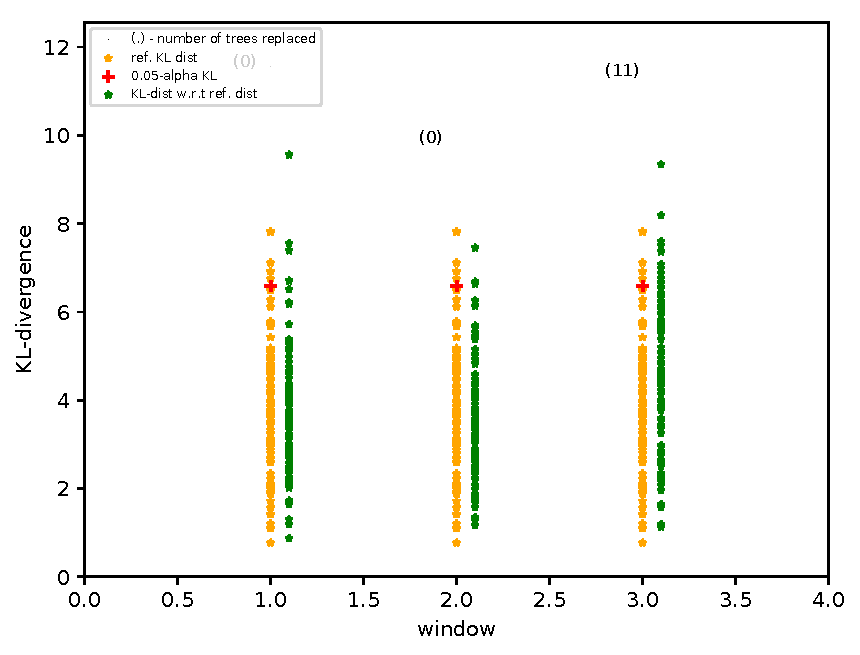
\includegraphics[width=\textwidth]{figures/test_concept_drift_abalone}
		\caption{Abalone}
		\label{fig:concept_drift_abalone}
	\end{subfigure}
	~ %add desired spacing between images, e. g. ~, \quad, \qquad, \hfill etc. 
	%(or a blank line to force the subfigure onto a new line)
	\begin{subfigure}[b]{0.23\textwidth}
		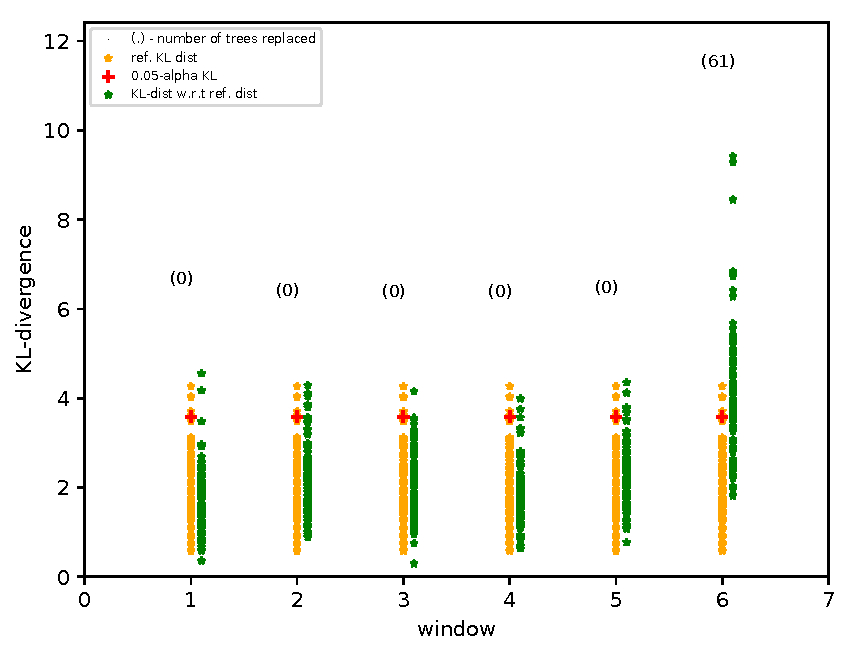
\includegraphics[width=\textwidth]{figures/test_concept_drift_ann_thyroid_1v3}
		\caption{ANN-Thyroid-1v3}
		\label{fig:concept_drift_ann_thyroid}
	\end{subfigure}
	~ %add desired spacing between images, e. g. ~, \quad, \qquad, \hfill etc. 
	%(or a blank line to force the subfigure onto a new line)
	\begin{subfigure}[b]{0.23\textwidth}
		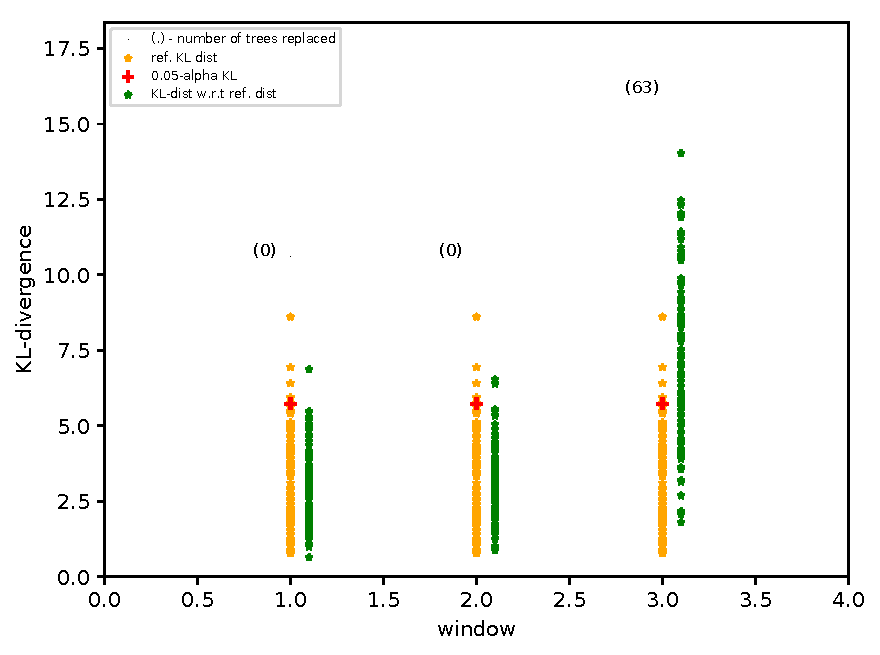
\includegraphics[width=\textwidth]{figures/test_concept_drift_cardiotocography_1}
		\caption{Cardiotocography}
		\label{fig:test_concept_drift_cardiotocography}
	\end{subfigure}
    ~ %add desired spacing between images, e. g. ~, \quad, \qquad, \hfill etc. 
    %(or a blank line to force the subfigure onto a new line)
    \begin{subfigure}[b]{0.23\textwidth}
    	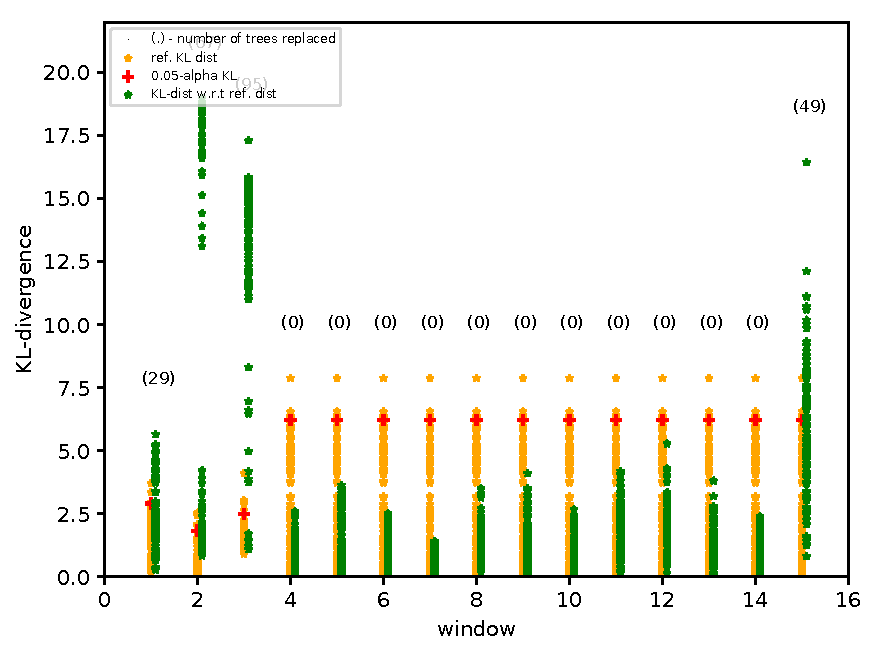
\includegraphics[width=\textwidth]{figures/test_concept_drift_kddcup}
    	\caption{KDDCup99}
    	\label{fig:concept_drift_kddcup}
    \end{subfigure} \\
    \begin{subfigure}[b]{0.23\textwidth}
    	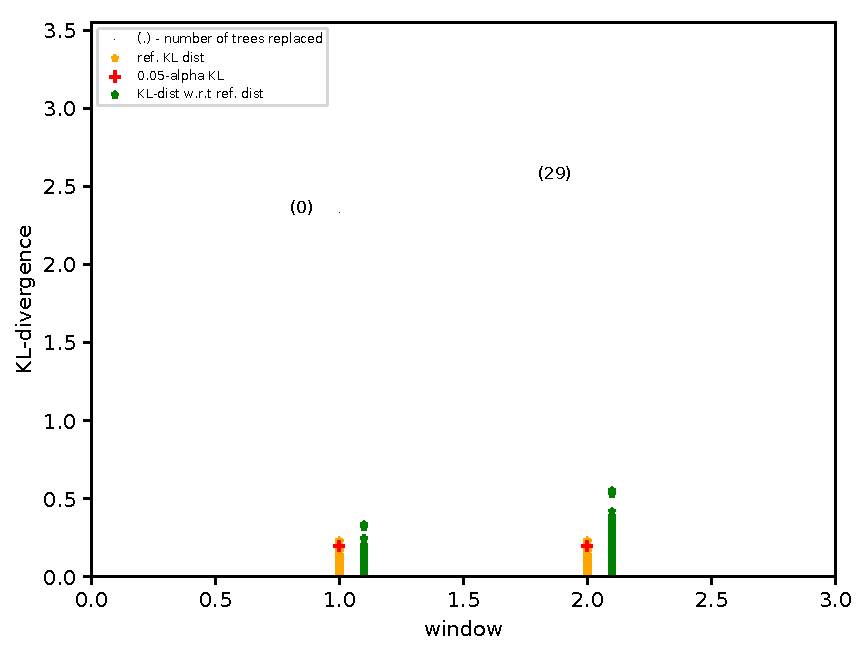
\includegraphics[width=\textwidth]{figures/test_concept_drift_mammography}
    	\caption{Mammography}
    	\label{fig:concept_drift_mammography}
    \end{subfigure}
    ~ %add desired spacing between images, e. g. ~, \quad, \qquad, \hfill etc. 
    %(or a blank line to force the subfigure onto a new line)
    \begin{subfigure}[b]{0.23\textwidth}
    	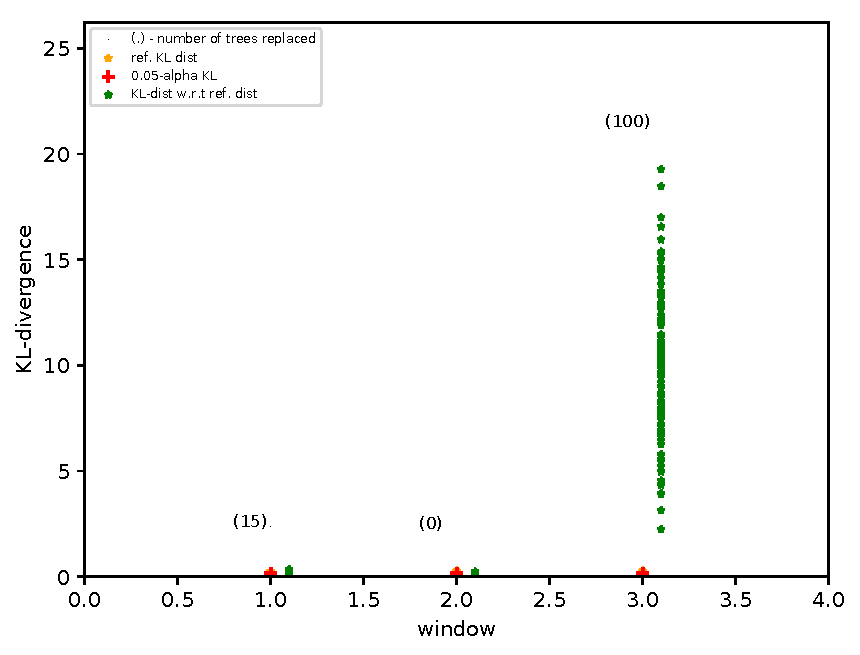
\includegraphics[width=\textwidth]{figures/test_concept_drift_shuttle_1v23567}
    	\caption{Shuttle}
    	\label{fig:concept_drift_shuttle}
    \end{subfigure}
    ~ %add desired spacing between images, e. g. ~, \quad, \qquad, \hfill etc. 
    %(or a blank line to force the subfigure onto a new line)
    \begin{subfigure}[b]{0.23\textwidth}
    	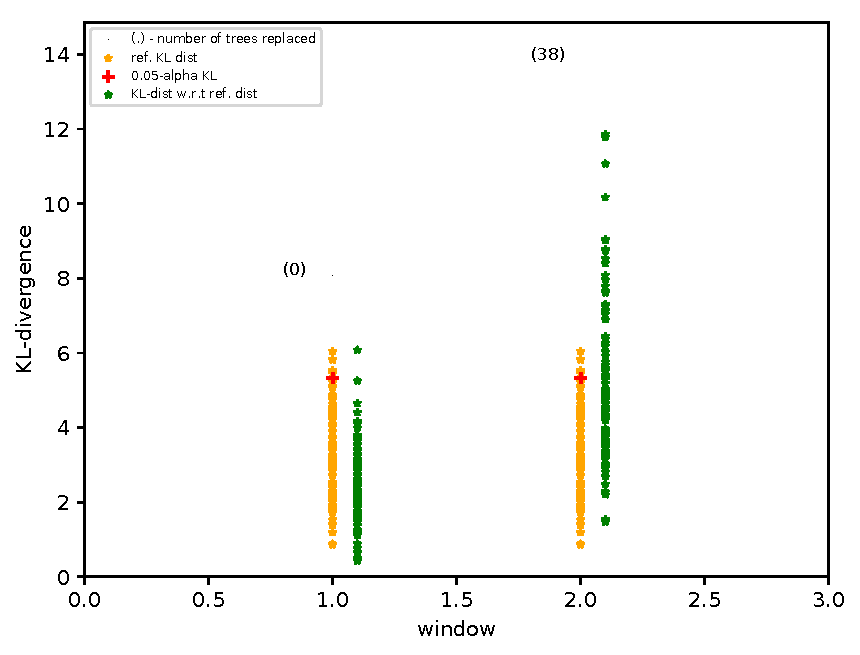
\includegraphics[width=\textwidth]{figures/test_concept_drift_yeast}
    	\caption{Yeast}
    	\label{fig:concept_drift_yeast}
    \end{subfigure}
    ~ %add desired spacing between images, e. g. ~, \quad, \qquad, \hfill etc. 
    %(or a blank line to force the subfigure onto a new line)
    \begin{subfigure}[b]{0.23\textwidth}
    	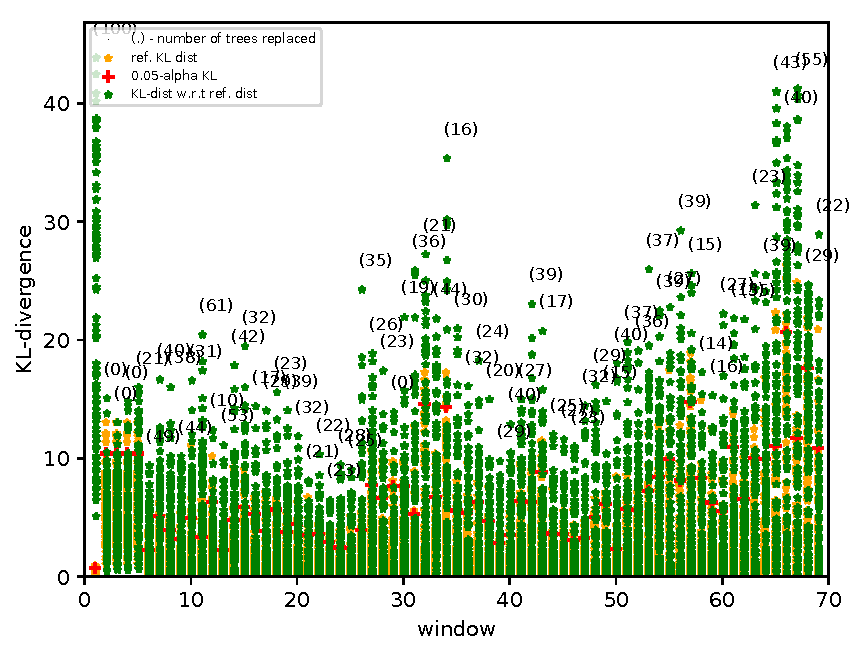
\includegraphics[width=\textwidth]{figures/test_concept_drift_covtype}
    	\caption{Covtype}
    	\label{fig:concept_drift_covtype}
    \end{subfigure} \\
    \begin{subfigure}[b]{0.23\textwidth}
      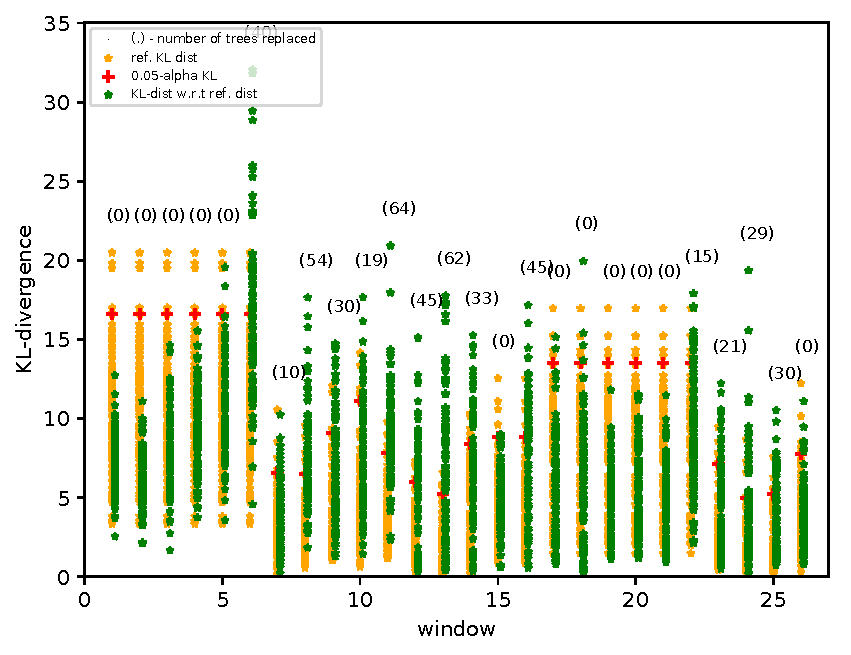
\includegraphics[width=\textwidth]{figures/test_concept_drift_electricity}
      \caption{Electricity}
      \label{fig:concept_drift_electricity}
    \end{subfigure}
    ~ %add desired spacing between images, e. g. ~, \quad, \qquad, \hfill etc. 
    %(or a blank line to force the subfigure onto a new line)
    \begin{subfigure}[b]{0.23\textwidth}
      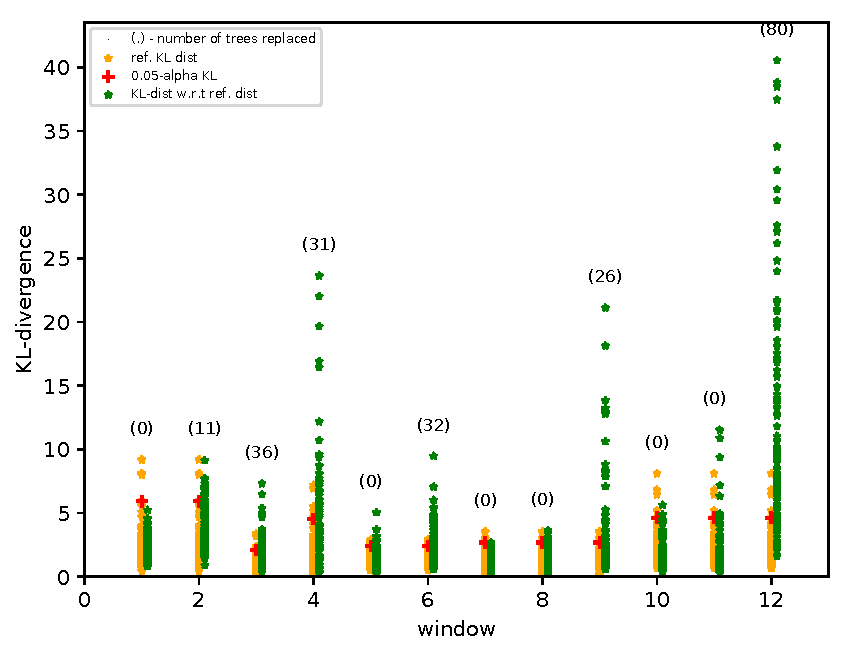
\includegraphics[width=\textwidth]{figures/test_concept_drift_weather}
      \caption{Weather}
      \label{fig:concept_drift_weather}
    \end{subfigure}
	\caption{Concept drift detection in datasets using tree-structures. The total number of trees in the forest model is held constant at ${\bf 100}$ for all datasets. Each dataset has a streaming window size commensurate with its total size: \textit{Abalone}($512$), \textit{ANN-Thyroid-1v3}($512$), \textit{Cardiotocography}($512$), \textit{Covtype}($4096$), \textit{Electricity}($1024$), \textit{KDDCup99}($4096$), \textit{Mammography}($4096$), \textit{Shuttle}($4096$), \textit{Weather}($1024$), and \textit{Yeast}($512$). The last data window in each dataset usually has much fewer instances and therefore its distribution is very different from the previous window despite there being no data drift. \textbf{Therefore, ignore the drift in the last window.} We did not expect \textit{Abalone}, \textit{ANN-Thyroid-1v3}, \textit{Cardiotocography}, \textit{KDDCup99}, \textit{Mammography}, \textit{Shuttle}, and \textit{Yeast} to have much drift in data, and this can also be seen in the plots where most of the windows in the middle of streaming did not result in too many trees being replaced (the numbers in the parenthesis are mostly zero). We also did not expect \textit{Covtype} to have much drift in its default ordering (from its public repository); however, after seeing the plots we realize that there is a definite drift due to which a significant number of trees need to be replaced with each new window of data. \textit{Electricity} and \textit{Weather} are standard streaming datasets with expected concept drift, which shows up in the plots.} \label{fig:concept_drift}
\end{figure}

\begin{figure}
	\centering
	\captionsetup{labelformat=empty}
	\begin{subfigure}[b]{0.3\textwidth}
		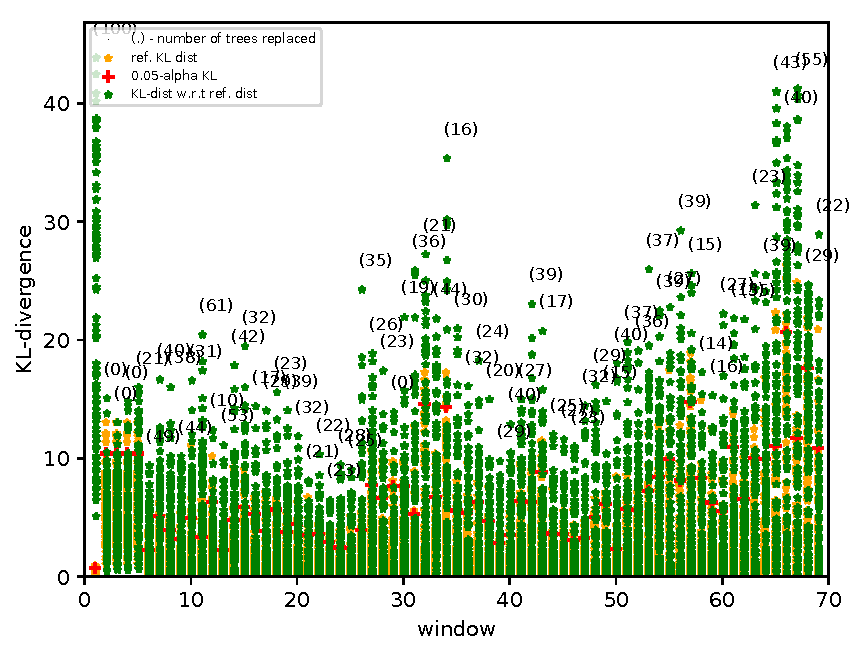
\includegraphics[width=\textwidth]{figures/test_concept_drift_covtype}
		\caption{Covtype}
		\label{fig:concept_drift_covtype_}
	\end{subfigure}
	\begin{subfigure}[b]{0.3\textwidth}
		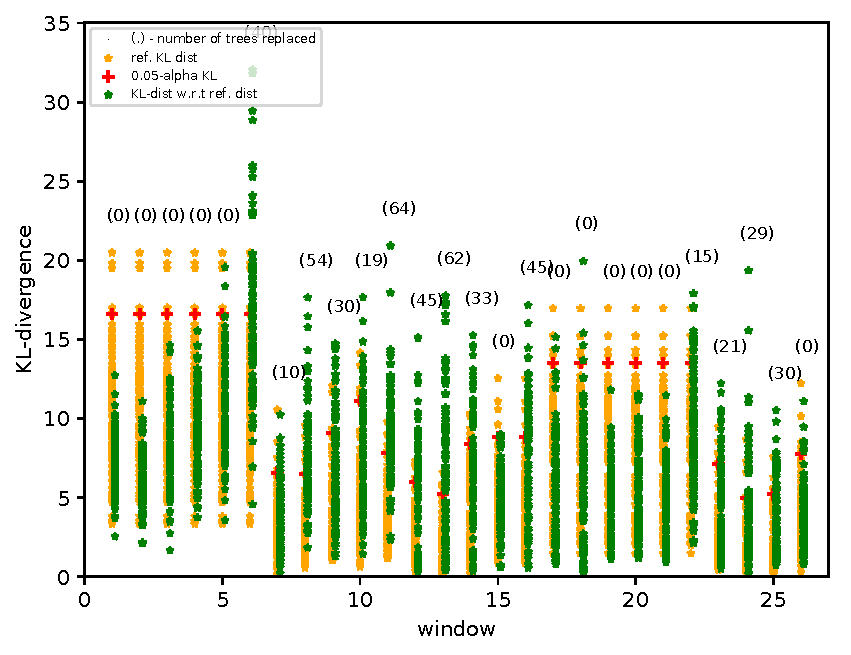
\includegraphics[width=\textwidth]{figures/test_concept_drift_electricity}
		\caption{Electricity}
		\label{fig:concept_drift_electricity_}
	\end{subfigure}
	~ %add desired spacing between images, e. g. ~, \quad, \qquad, \hfill etc. 
	%(or a blank line to force the subfigure onto a new line)
	\begin{subfigure}[b]{0.3\textwidth}
		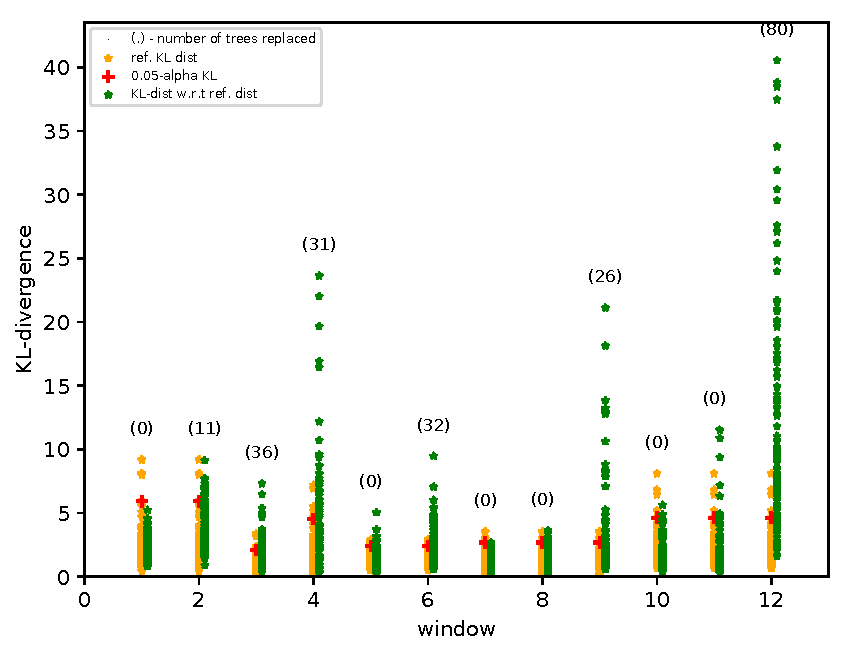
\includegraphics[width=\textwidth]{figures/test_concept_drift_weather}
		\caption{Weather}
		\label{fig:concept_drift_weather_}
	\end{subfigure} \\
    \begin{subfigure}[b]{0.3\textwidth}
    	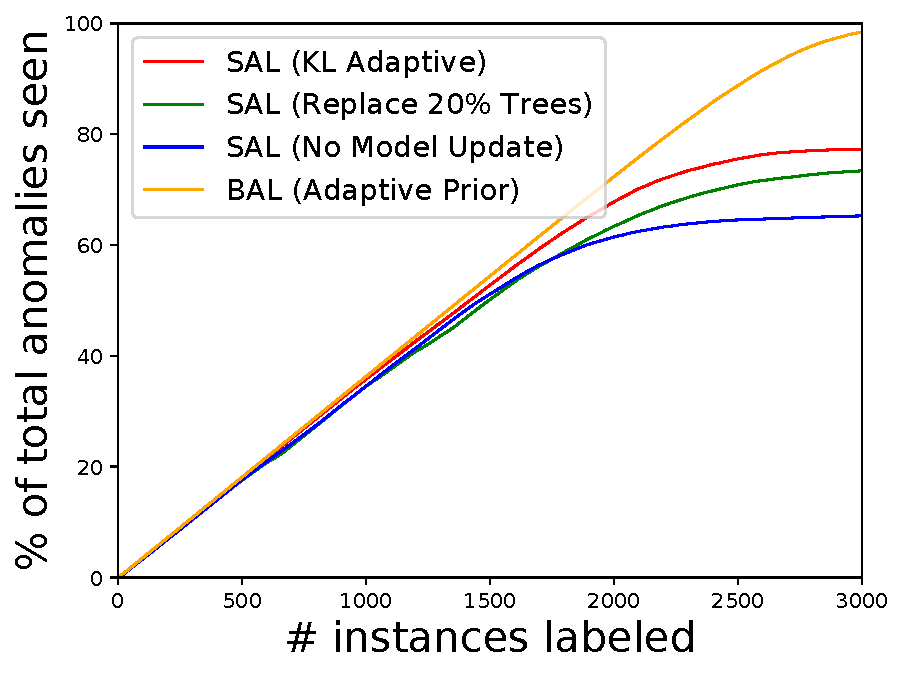
\includegraphics[width=\textwidth]{figures/num_seen-covtype}
    	\caption{Covtype}
    	\label{fig:concept_drift_covtype_num}
    \end{subfigure}
    \begin{subfigure}[b]{0.3\textwidth}
    	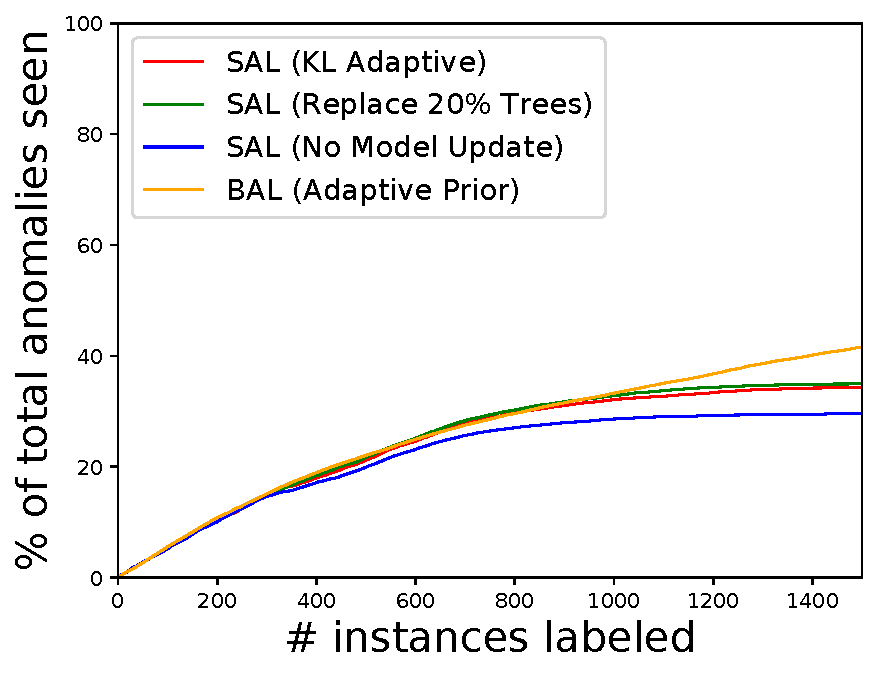
\includegraphics[width=\textwidth]{figures/num_seen-electricity}
    	\caption{Electricity}
    	\label{fig:concept_drift_electricity_num}
    \end{subfigure}
    ~ %add desired spacing between images, e. g. ~, \quad, \qquad, \hfill etc. 
    %(or a blank line to force the subfigure onto a new line)
    \begin{subfigure}[b]{0.3\textwidth}
    	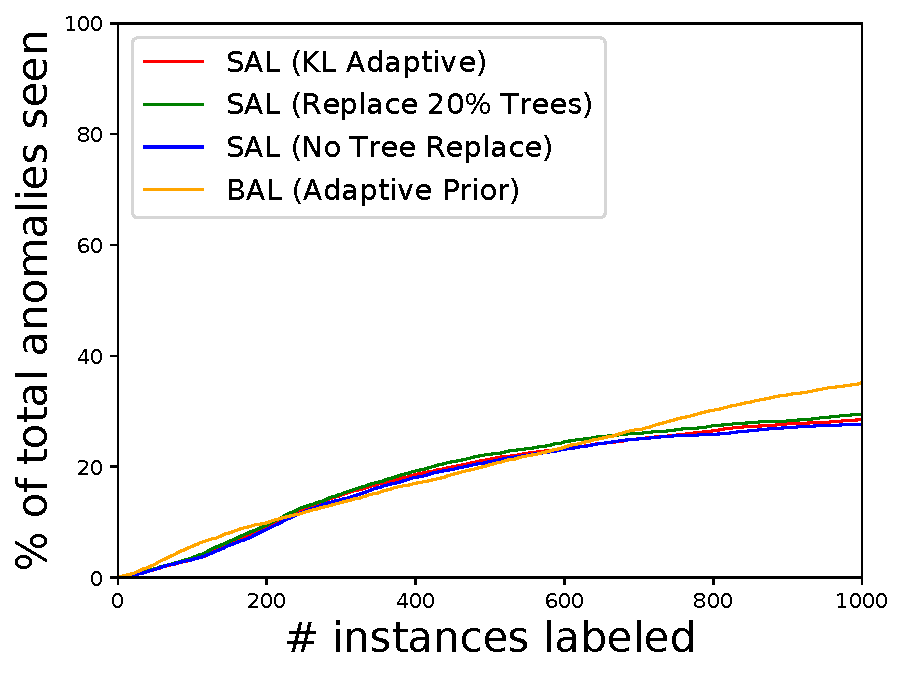
\includegraphics[width=\textwidth]{figures/num_seen-weather}
    	\caption{Weather}
    	\label{fig:concept_drift_weather_num}
    \end{subfigure}
	\caption{Integrated drift detection and label feedback with Stream Active Learner (SAL). The query budget and the stream window size for each dataset was set as: \textit{Covtype}($3000, 4096$), \textit{Electricity}($1500, 1024$), and \textit{Weather}($1000, 1024$). The max memory limit was set equal to the window size. We query $20$ labels every time a window of data arrives. The all remaining query budget is used with the final set of instances in memory after the last window has been processed. All experiments employed \textit{Retention Type 1} where only the most anomalous instances fitting the memory limit are retained in memory. When a new window of data arrives: \texttt{SAL~(KL~Adaptive)} dynamically determines which trees to replace, \texttt{SAL~(Replace 20\%~Trees)} replaces $20\%$ oldest trees, and \texttt{SAL~(No~Model~Update)} keeps the trees fixed after initially training with the first window of data. \texttt{BAL~(Adaptive~Prior)} is the Batch Active Learner without any memory limitation and is the most optimistic setup because all data is available in memory right from the start. \texttt{SAL~(KL~Adaptive)} \textbf{is the best performing streaming strategy} on these datasets and \textbf{also competitive} with \texttt{BAL~(Adaptive~Prior)}.} \label{fig:concept_drift_num}
\end{figure}

\iffalse
\begin{thebibliography}{1}
\bibitem{test:2018} Author One and Author Two {Test Reference},  2018, Venue.
\end{thebibliography}
\fi

\end{document}
